\chapter{Pixels detectors for the new ATLAS Inner Tracker}
\label{chap:ITk}

In this Chapter the new ATLAS Inner Tracker (ITk) of the ATLAS detector will be discussed. It is intended to be ready 
for  the data taking in 2026, in time for the beginning of the High Luminosity phase of the LHC (HL-LHC). 
The plans for the upgrades of the LHC are presented in Section~\ref{sec:HL-LHC}, along with the 
physics case and the ATLAS sub detector upgrades for the Phase-II; 
Section~\ref{sec:NewTracker} will cover the performance and specifications for the new ATLAS ITk. 
After describing the R\&D efforts for ITk pixels detectors in general (Section~\ref{sec:ITkPixels}), 
in Section~\ref{sec:radhardpixels} results for radiation hard pixel sensors will be presented. 
The concept of slim edge, already applied to IBL pixel sensors (Section~\ref{sec:IBLoverview}) will be 
pushed to its limits for the ITk pixels sensors; this topic will be discussed in details in 
Section~\ref{sec:edgeless}, together with results from beam tests. 
Eventually conclusions and perspectives will be drawn in Section~\ref{sec:itksummary}.



\section{High Luminosity LHC and the Phase-II of the LHC experiments}
\label{sec:HL-LHC}

The timeline of the CERN LHC is presented in Figure~\ref{fig:HL-LHC-plan-2016-01}, together 
with the future plans. The High Luminosity LHC (HL-LHC)~\cite{HL_LHC} is a project, recently 
approved~\cite{HL-LHCApproval},  to upgrade the existing LHC to a high luminosity machine, 
capable to deliver an instantaneous luminosity of $L=7.5\times10^{34}$/cm$^{2}$/s; as a 
reminder the design luminosity of LHC is of $L=1.0\times10^{34}$/cm$^{2}$/s.
\begin{figure}[!htpb]
\centering
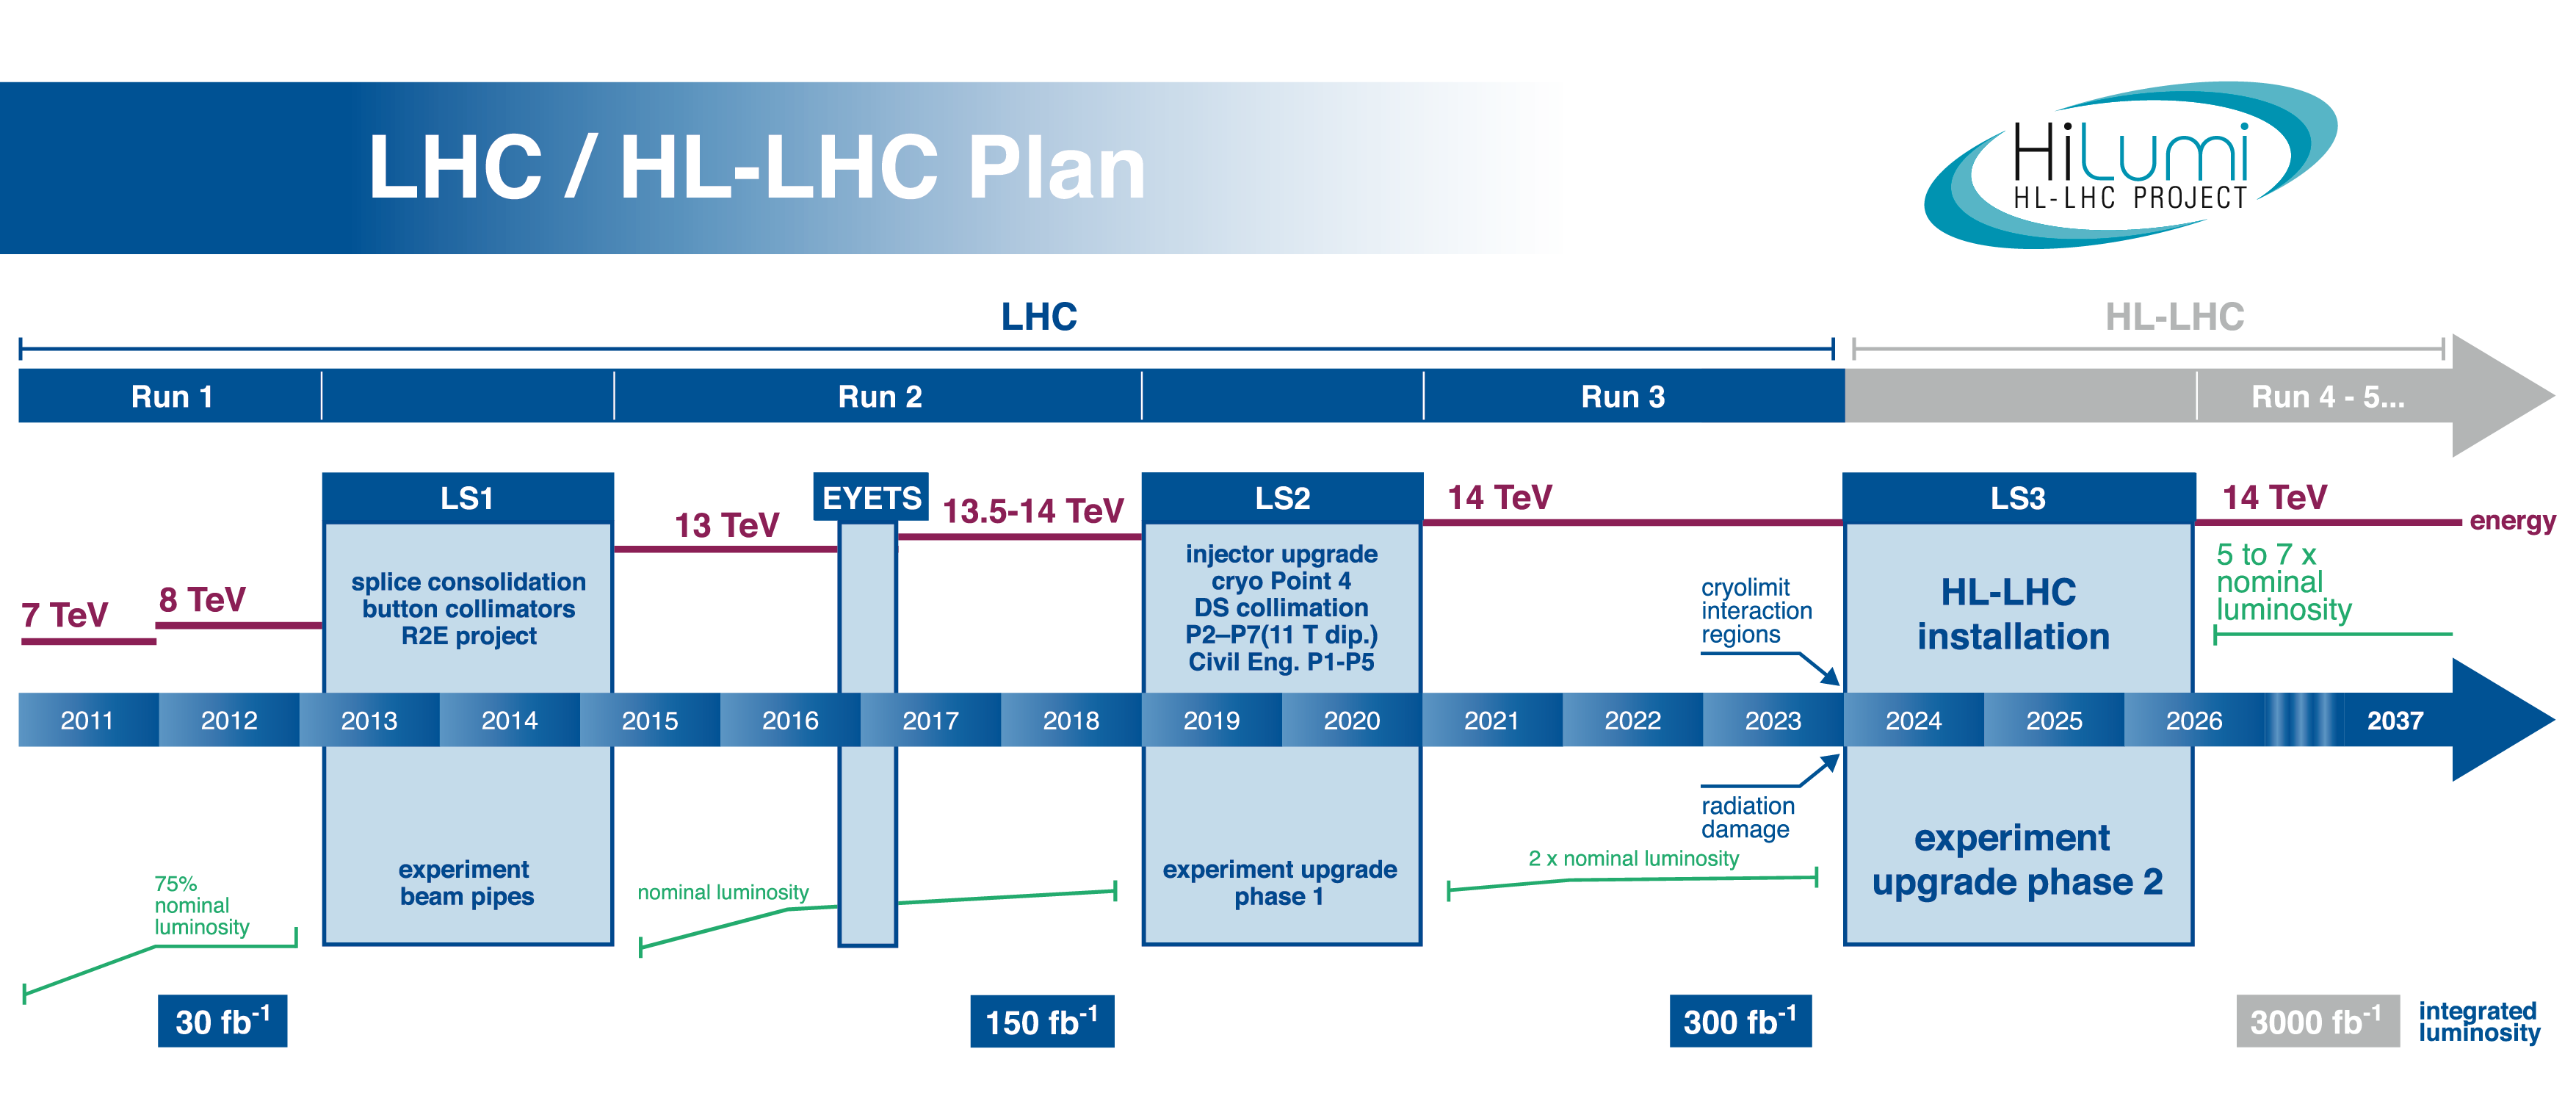
\includegraphics[width=1.0\textwidth]{HL-LHC-plan-2016-01.png}
\caption{\label{fig:HL-LHC-plan-2016-01}LHC/ HL-LHC Plan (last update 22.02.2016, after~\cite{HL_LHC})}
\end{figure}
After the HL-LHC upgrade completion the data taking  is expected to restart in 2026; the goal 
is to integrate a dataset of 3000~\invfb by 2037; there is an option to extend this program to arrive 
at 4000~\invfb.

As it can be seen in Figure~\ref{fig:HL-LHC-plan-2016-01} the upgrade plans don't include any increase 
of the center-of-mass energy $\sqrt{s}$. Thus, the main motivation for the HL-LHC project is 
reducing the error halving time. Indeed, taking data beyond 2023 at the same instantaneous luminosity of 
Run~3 would imply  to take data for more than 15 years to reduce the statistical error by a factor of 2.

The large dataset at the end of the so-called Phase 2 (or {\it} Phase-II) for the experiments should enable 
a  large program of precision measurements of the Higgs boson and discoveries. 
As an example of the potential of the HL-LHC dataset, the projected precision on coupling of the Higgs
 boson to $\mu$s is of about 7\% with  3000~\invfb; the Higgs 
trilinear self coupling parameter $\lambda_{HHH}$ can be probed at about 1 $\sigma$ significance 
in the range $-0.8<\lambda_{HHH}/\lambda_{SM}<7.7$ ($\lambda_{SM}$ is the SM predicted value) 
in the final state $HH\to\b\bbar\gamma\gamma$~\cite{ATL-PHYS-PUB-2014-016}. 
For what concerns physics beyond SM (BSM), the supersymmetric\footnote{Supersymmetry (SUSY) is a proposed type of spacetime symmetry where  each SM particle is associated with another particle, known as its superpartner, the spin of which differs by a half-integer; for an introduction to SUSY~\cite{SusyPrimer}} top quark partner $\widetilde{t}$, 
the {\it stop}, discovery mass range is up to 480~GeV, and an exclusion one to 700~GeV~\cite{ATL-PHYS-PUB-2016-022} with the HL-LHC dataset; with the same amount of data the SUSY partners of Higgs and 
vector bosons, the so-called charginos and neutralinos, can be investigated up to about 1~TeV of mass, 
and excluded up to 1.3~TeV~\cite{ATL-PHYS-PUB-2015-032}. Other than SUSY the physics program 
during the Phase-II of the LHC experiments include searches of higher  vector bosons resonances like 
$W',Z'$, 
extra dimensions and more~\cite{ATLASLoIPhaseII}.

The high luminosity foreseen for the Phase-II implies a much harsher environment than in Run~2 
for the ATLAS sub-detectors; indeed high luminosity means higher event rate, more pileup events 
and higher radiation doses and fluences. 
To cope with the severe data taking conditions expected at the HL-LHC it is planned to 
upgrade the  ATLAS detector~\cite{ATLASLoIPhaseII,ATLASITkScopingDocument}. Upgrades include:

\begin{itemize}
\item a longer latency trigger system, to cope with higher event rates,
\item new inner muon barrel trigger chambers, to assure redundancy and improve efficiency,
\item the upgrade of the tile calorimeter electronics, since the actual system will not survive he doses expected by the time of HL-LHC and
\item a complete new silicon only tracker, with coverage down to pseudorapidity $|\eta|=4$, the {\it Inner Tracker} (ITk)
\end{itemize} 

The constraints, requirements, layout and expected performance of the proposed ATLAS ITk will 
be discussed in the next Section.

\section{The Quest for a New ATLAS Inner Tracker}
\label{sec:NewTracker}

The new ATLAS  Inner Tracker will have to face unprecedented levels of radiation doses and fluences, 
pileup events and events rate. Table~\ref{tab:ITkConditions} summarises the most important figures.

\begin{table}[!htpb]
\centering
\caption{\label{tab:ITkConditions}Environment conditions for the inner detector at the LHC and HL-LHC}
\begin{tabular}{lcc}
\hline
\hline
Parameter & LHC & HL-LHC \\
\hline
instantaneous luminosity $L$	 [cm$^{-2}$s$^{-1}$] & $1.0\times10^{34}$ &  $7.5\times10^{34}$ \\
number of pileup events $\mu$ & 25 & 200\\
fluence to the innermost pixel layer $\Phi$ [ 1 MeV $n_\text{eq}/\text{cm}^2$] & 5$\times10^{15}$ & 2$\times10^{16}$ \\

\end{tabular}
\end{table}

\section{Pixels Detectors for ITK}
\label{sec:ITkPixels}

\section{Radiation Hard Pixel Sensors}
\label{sec:radhardpixels}
\section{Edgeless Pixel Sensors}
\label{sec:edgeless}

\section{Summary and Outlook}
\label{sec:itksummary}

